% NHSJS-format skeleton. Build with:  python3 build.py   (writes nhsjs_standard.pdf and nhsjs_online.pdf)
% The grey NOTES boxes list facts and numbers only. Replace each box with prose you write yourselves,
% then delete the box. Do not paste sentences from the arXiv version: see README.md in this folder.
\documentclass[12pt,a4paper]{article}
\usepackage[T1]{fontenc}
\usepackage[utf8]{inputenc}
\usepackage{lmodern}
\usepackage[margin=2.5cm]{geometry}
\usepackage{amsmath,graphicx,booktabs,array,caption,enumitem,xcolor,framed}
\usepackage[section]{placeins}
\usepackage[hidelinks]{hyperref}
\usepackage{xurl}
\captionsetup{font=small,labelfont=bf}
\setlist{itemsep=1pt,topsep=3pt}
\expandafter\def\csname res@Tc\endcsname{3272}
\expandafter\def\csname res@altApForty\endcsname{227}
\expandafter\def\csname res@altApTwenty\endcsname{190}
\expandafter\def\csname res@altGainHigh\endcsname{1.3}
\expandafter\def\csname res@altGainLow\endcsname{2.4}
\expandafter\def\csname res@altVForty\endcsname{240\,000}
\expandafter\def\csname res@altVTwenty\endcsname{4\,500}
\expandafter\def\csname res@altVolRatioHigh\endcsname{8.9}
\expandafter\def\csname res@altVolRatioLow\endcsname{6.0}
\expandafter\def\csname res@atmP\endcsname{1197}
\expandafter\def\csname res@atmRho\endcsname{0.0184}
\expandafter\def\csname res@atmT\endcsname{226.5}
\expandafter\def\csname res@audDiv\endcsname{60.45}
\expandafter\def\csname res@audDvBack\endcsname{2173}
\expandafter\def\csname res@audDvPct\endcsname{24}
\expandafter\def\csname res@audEratio\endcsname{34}
\expandafter\def\csname res@audGasRatio\endcsname{11.5}
\expandafter\def\csname res@audH2ratio\endcsname{70}
\expandafter\def\csname res@audLnA\endcsname{0.916}
\expandafter\def\csname res@audLnB\endcsname{1.253}
\expandafter\def\csname res@audMolar\endcsname{947}
\expandafter\def\csname res@audPratio\endcsname{9.8}
\expandafter\def\csname res@audRhoLow\endcsname{1.8}
\expandafter\def\csname res@audRhoRatio\endcsname{10.4}
\expandafter\def\csname res@audRhoTot\endcsname{56}
\expandafter\def\csname res@audVolRatio\endcsname{6.1}
\expandafter\def\csname res@balAp\endcsname{214}
\expandafter\def\csname res@balArea\endcsname{4347}
\expandafter\def\csname res@balBareH2\endcsname{22.5}
\expandafter\def\csname res@balBareV\endcsname{17\,600}
\expandafter\def\csname res@balDv\endcsname{2091}
\expandafter\def\csname res@balEnv\endcsname{130}
\expandafter\def\csname res@balEps\endcsname{36.4}
\expandafter\def\csname res@balF\endcsname{11.8}
\expandafter\def\csname res@balH2\endcsname{34.5}
\expandafter\def\csname res@balHb\endcsname{58.0}
\expandafter\def\csname res@balHe\endcsname{75.4}
\expandafter\def\csname res@balHeMassRatio\endcsname{2.18}
\expandafter\def\csname res@balHeVolPct\endcsname{10}
\expandafter\def\csname res@balIsp\endcsname{303.4}
\expandafter\def\csname res@balIspVac\endcsname{307.3}
\expandafter\def\csname res@balLaunchH2\endcsname{38}
\expandafter\def\csname res@balLd\endcsname{8}
\expandafter\def\csname res@balLg\endcsname{369}
\expandafter\def\csname res@balMdot\endcsname{3.97}
\expandafter\def\csname res@balPe\endcsname{4.7}
\expandafter\def\csname res@balQ\endcsname{1.7}
\expandafter\def\csname res@balTap\endcsname{222}
\expandafter\def\csname res@balTb\endcsname{38.1}
\expandafter\def\csname res@balV\endcsname{27\,000}
\expandafter\def\csname res@balVHe\endcsname{29\,600}
\expandafter\def\csname res@balVHi\endcsname{30\,300}
\expandafter\def\csname res@balVLo\endcsname{24\,000}
\expandafter\def\csname res@balVb\endcsname{1714}
\expandafter\def\csname res@betaBase\endcsname{2397}
\expandafter\def\csname res@betaHi\endcsname{4506}
\expandafter\def\csname res@betaLo\endcsname{1046}
\expandafter\def\csname res@bmCstar\endcsname{1726}
\expandafter\def\csname res@bmFrozen\endcsname{274.9}
\expandafter\def\csname res@bmShift\endcsname{285.9}
\expandafter\def\csname res@bmTc\endcsname{3426}
\expandafter\def\csname res@cBalD\endcsname{0.31}
\expandafter\def\csname res@cBalDry\endcsname{90.4}
\expandafter\def\csname res@cBalEnv\endcsname{89}
\expandafter\def\csname res@cBalF\endcsname{5.5}
\expandafter\def\csname res@cBalGas\endcsname{19.3}
\expandafter\def\csname res@cBalM\endcsname{140}
\expandafter\def\csname res@cBalMSS\endcsname{168}
\expandafter\def\csname res@cBalMp\endcsname{49.6}
\expandafter\def\csname res@cBalTb\endcsname{27.1}
\expandafter\def\csname res@cBalV\endcsname{15\,100}
\expandafter\def\csname res@cGndM\endcsname{348}
\expandafter\def\csname res@cGndMSS\endcsname{755}
\expandafter\def\csname res@cGndMp\endcsname{222}
\expandafter\def\csname res@cMassRatio\endcsname{2.5}
\expandafter\def\csname res@cPropRatio\endcsname{4.5}
\expandafter\def\csname res@cSysBal\endcsname{280}
\expandafter\def\csname res@cTwentyM\endcsname{152}
\expandafter\def\csname res@cTwentyV\endcsname{2\,500}
\expandafter\def\csname res@cstar\endcsname{1720}
\expandafter\def\csname res@deaCdFit\endcsname{1.16}
\expandafter\def\csname res@deaD\endcsname{0.171}
\expandafter\def\csname res@deaDragShare\endcsname{8}
\expandafter\def\csname res@deaErrCold\endcsname{+6.2}
\expandafter\def\csname res@deaErrMaxAbs\endcsname{2.6}
\expandafter\def\csname res@deaErrMean\endcsname{+1.3}
\expandafter\def\csname res@deaGroundHeavy\endcsname{22}
\expandafter\def\csname res@deaGroundLight\endcsname{25}
\expandafter\def\csname res@deaImp\endcsname{87.5}
\expandafter\def\csname res@deaIsp\endcsname{191}
\expandafter\def\csname res@deaMp\endcsname{46.7}
\expandafter\def\csname res@deaRmsFit\endcsname{0.8}
\expandafter\def\csname res@deaRmsUnit\endcsname{1.4}
\expandafter\def\csname res@decAltTenBal\endcsname{127}
\expandafter\def\csname res@decAltTenDrag\endcsname{63}
\expandafter\def\csname res@decAltTenGnd\endcsname{35}
\expandafter\def\csname res@decAltTenHead\endcsname{11}
\expandafter\def\csname res@decAltTenNozzle\endcsname{26}
\expandafter\def\csname res@decAltTenRatio\endcsname{3.7}
\expandafter\def\csname res@decAltTwentyBal\endcsname{190}
\expandafter\def\csname res@decAltTwentyDrag\endcsname{56}
\expandafter\def\csname res@decAltTwentyGnd\endcsname{35}
\expandafter\def\csname res@decAltTwentyHead\endcsname{13}
\expandafter\def\csname res@decAltTwentyNozzle\endcsname{31}
\expandafter\def\csname res@decAltTwentyRatio\endcsname{5.5}
\expandafter\def\csname res@decDrag\endcsname{93}
\expandafter\def\csname res@decFDrag\endcsname{52}
\expandafter\def\csname res@decFHead\endcsname{17}
\expandafter\def\csname res@decFNozzle\endcsname{31}
\expandafter\def\csname res@decHead\endcsname{31}
\expandafter\def\csname res@decMassBigBal\endcsname{203}
\expandafter\def\csname res@decMassBigDrag\endcsname{41}
\expandafter\def\csname res@decMassBigGnd\endcsname{60}
\expandafter\def\csname res@decMassBigHead\endcsname{22}
\expandafter\def\csname res@decMassBigNozzle\endcsname{37}
\expandafter\def\csname res@decMassBigRatio\endcsname{3.4}
\expandafter\def\csname res@decMassFiftyBal\endcsname{221}
\expandafter\def\csname res@decMassFiftyDrag\endcsname{60}
\expandafter\def\csname res@decMassFiftyGnd\endcsname{18}
\expandafter\def\csname res@decMassFiftyHead\endcsname{15}
\expandafter\def\csname res@decMassFiftyNozzle\endcsname{24}
\expandafter\def\csname res@decMassFiftyRatio\endcsname{12.4}
\expandafter\def\csname res@decNozzle\endcsname{56}
\expandafter\def\csname res@dryFor100\endcsname{269}
\expandafter\def\csname res@dvCap\endcsname{991}
\expandafter\def\csname res@dvCapOpt\endcsname{1235}
\expandafter\def\csname res@fallAp\endcsname{181}
\expandafter\def\csname res@fallCost\endcsname{33}
\expandafter\def\csname res@fallDv\endcsname{2086}
\expandafter\def\csname res@fallEps\endcsname{36.4}
\expandafter\def\csname res@fallF\endcsname{11.8}
\expandafter\def\csname res@fallHb\endcsname{51.5}
\expandafter\def\csname res@fallIsp\endcsname{302.8}
\expandafter\def\csname res@fallIspVac\endcsname{307.3}
\expandafter\def\csname res@fallLd\endcsname{10}
\expandafter\def\csname res@fallLg\endcsname{369}
\expandafter\def\csname res@fallMdot\endcsname{3.98}
\expandafter\def\csname res@fallPe\endcsname{4.7}
\expandafter\def\csname res@fallQ\endcsname{2.2}
\expandafter\def\csname res@fallSpeed\endcsname{139}
\expandafter\def\csname res@fallTap\endcsname{205}
\expandafter\def\csname res@fallTb\endcsname{38.0}
\expandafter\def\csname res@fallVb\endcsname{1567}
\expandafter\def\csname res@feedAl\endcsname{0.211}
\expandafter\def\csname res@feedSS\endcsname{0.477}
\expandafter\def\csname res@filmAreal\endcsname{18.4}
\expandafter\def\csname res@frDeficitPct\endcsname{15}
\expandafter\def\csname res@frDel\endcsname{246}
\expandafter\def\csname res@frFrozen\endcsname{241.4}
\expandafter\def\csname res@frShift\endcsname{267.9}
\expandafter\def\csname res@frTc\endcsname{1443}
\expandafter\def\csname res@ftAl\endcsname{0.060}
\expandafter\def\csname res@ftHP\endcsname{1.97}
\expandafter\def\csname res@ftSS\endcsname{0.237}
\expandafter\def\csname res@gainKm\endcsname{179}
\expandafter\def\csname res@gainRatio\endcsname{6.2}
\expandafter\def\csname res@gasH2\endcsname{0.0748}
\expandafter\def\csname res@gasHe\endcsname{0.160}
\expandafter\def\csname res@gndAp\endcsname{35}
\expandafter\def\csname res@gndDv\endcsname{1636}
\expandafter\def\csname res@gndEps\endcsname{3.68}
\expandafter\def\csname res@gndF\endcsname{11.8}
\expandafter\def\csname res@gndFirstTen\endcsname{9.2}
\expandafter\def\csname res@gndHb\endcsname{11.7}
\expandafter\def\csname res@gndIsp\endcsname{226.4}
\expandafter\def\csname res@gndIspVac\endcsname{259.0}
\expandafter\def\csname res@gndLd\endcsname{508}
\expandafter\def\csname res@gndLg\endcsname{278}
\expandafter\def\csname res@gndMdot\endcsname{5.32}
\expandafter\def\csname res@gndPe\endcsname{106.0}
\expandafter\def\csname res@gndQ\endcsname{121}
\expandafter\def\csname res@gndTap\endcsname{95}
\expandafter\def\csname res@gndTb\endcsname{28.4}
\expandafter\def\csname res@gndVb\endcsname{850}
\expandafter\def\csname res@h2oRatio\endcsname{6}
\expandafter\def\csname res@heBottleHi\endcsname{2.6}
\expandafter\def\csname res@heBottleKg\endcsname{0.113}
\expandafter\def\csname res@heBottleLo\endcsname{1.4}
\expandafter\def\csname res@heBottleMid\endcsname{1.8}
\expandafter\def\csname res@heKg\endcsname{0.0085}
\expandafter\def\csname res@heMassHi\endcsname{50}
\expandafter\def\csname res@heMassLo\endcsname{26}
\expandafter\def\csname res@heMassMid\endcsname{34}
\expandafter\def\csname res@heVolHi\endcsname{872}
\expandafter\def\csname res@heVolLo\endcsname{453}
\expandafter\def\csname res@heVolMid\endcsname{597}
\expandafter\def\csname res@ispDel\endcsname{307.3}
\expandafter\def\csname res@ispDelHi\endcsname{317}
\expandafter\def\csname res@ispDelLo\endcsname{284}
\expandafter\def\csname res@ispFrozen\endcsname{312.9}
\expandafter\def\csname res@ispFrozenPeak\endcsname{315.0}
\expandafter\def\csname res@ispShift\endcsname{334.0}
\expandafter\def\csname res@ispShiftPeak\endcsname{335.8}
\expandafter\def\csname res@lapP\endcsname{270}
\expandafter\def\csname res@lapRho\endcsname{0.0101}
\expandafter\def\csname res@lapT\endcsname{93.45}
\expandafter\def\csname res@lapZero\endcsname{44}
\expandafter\def\csname res@mapApTen\endcsname{127}
\expandafter\def\csname res@mcBalCv\endcsname{9}
\expandafter\def\csname res@mcBalHi\endcsname{238}
\expandafter\def\csname res@mcBalLo\endcsname{176}
\expandafter\def\csname res@mcBalMed\endcsname{204}
\expandafter\def\csname res@mcDragLargest\endcsname{100}
\expandafter\def\csname res@mcFDragHi\endcsname{56}
\expandafter\def\csname res@mcFDragLo\endcsname{46}
\expandafter\def\csname res@mcFDragMed\endcsname{51}
\expandafter\def\csname res@mcFHeadHi\endcsname{21}
\expandafter\def\csname res@mcFHeadLo\endcsname{16}
\expandafter\def\csname res@mcFHeadMed\endcsname{18}
\expandafter\def\csname res@mcFNozzleHi\endcsname{34}
\expandafter\def\csname res@mcFNozzleLo\endcsname{27}
\expandafter\def\csname res@mcFNozzleMed\endcsname{30}
\expandafter\def\csname res@mcGndCv\endcsname{18}
\expandafter\def\csname res@mcGndHi\endcsname{43}
\expandafter\def\csname res@mcGndLo\endcsname{24}
\expandafter\def\csname res@mcGndMed\endcsname{32}
\expandafter\def\csname res@mcN\endcsname{10\,000}
\expandafter\def\csname res@mcNshap\endcsname{1\,000}
\expandafter\def\csname res@mcPbelow\endcsname{0.0}
\expandafter\def\csname res@mcRatioHi\endcsname{8.0}
\expandafter\def\csname res@mcRatioLo\endcsname{5.0}
\expandafter\def\csname res@mcRatioMed\endcsname{6.3}
\expandafter\def\csname res@mpFor100\endcsname{82}
\expandafter\def\csname res@mrCap\endcsname{1.51}
\expandafter\def\csname res@nacaMassHi\endcsname{106}
\expandafter\def\csname res@nacaMassLo\endcsname{86}
\expandafter\def\csname res@ofFrozenPeak\endcsname{2.05}
\expandafter\def\csname res@ofShiftPeak\endcsname{2.75}
\expandafter\def\csname res@peakAccel\endcsname{8.1}
\expandafter\def\csname res@propFrac\endcsname{0.502}
\expandafter\def\csname res@propH2Ratio\endcsname{7.5}
\expandafter\def\csname res@propRhoOwn\endcsname{0.099}
\expandafter\def\csname res@propVolL\endcsname{156}
\expandafter\def\csname res@propVolRatio\endcsname{9.4}
\expandafter\def\csname res@rhoBalCd\endcsname{-0.02}
\expandafter\def\csname res@rhoBalDry\endcsname{-0.70}
\expandafter\def\csname res@rhoBalEta\endcsname{+0.66}
\expandafter\def\csname res@rhoBalTw\endcsname{+0.20}
\expandafter\def\csname res@rhoBalZf\endcsname{+0.10}
\expandafter\def\csname res@rhoGndCd\endcsname{-0.70}
\expandafter\def\csname res@rhoGndDry\endcsname{-0.31}
\expandafter\def\csname res@rhoGndEta\endcsname{+0.58}
\expandafter\def\csname res@rhoGndTw\endcsname{-0.23}
\expandafter\def\csname res@rhoGndZf\endcsname{-0.01}
\expandafter\def\csname res@rhoH2float\endcsname{0.00128}
\expandafter\def\csname res@runBBB\endcsname{214}
\expandafter\def\csname res@runBBG\endcsname{144}
\expandafter\def\csname res@runBGB\endcsname{106}
\expandafter\def\csname res@runBGG\endcsname{65}
\expandafter\def\csname res@runGBB\endcsname{182}
\expandafter\def\csname res@runGBG\endcsname{112}
\expandafter\def\csname res@runGGB\endcsname{75}
\expandafter\def\csname res@runGGG\endcsname{35}
\expandafter\def\csname res@sCdHi\endcsname{212}
\expandafter\def\csname res@sCdLo\endcsname{215}
\expandafter\def\csname res@sEtaHi\endcsname{227}
\expandafter\def\csname res@sEtaLo\endcsname{185}
\expandafter\def\csname res@sGndCdHi\endcsname{28}
\expandafter\def\csname res@sGndCdLo\endcsname{43}
\expandafter\def\csname res@sGndD30\endcsname{58}
\expandafter\def\csname res@sGndD35\endcsname{45}
\expandafter\def\csname res@sTwHi\endcsname{221}
\expandafter\def\csname res@sTwLo\endcsname{176}
\expandafter\def\csname res@suiApHeavy\endcsname{60}
\expandafter\def\csname res@suiApLight\endcsname{91}
\expandafter\def\csname res@suiFire\endcsname{11.6}
\expandafter\def\csname res@suiMassFit\endcsname{103}
\expandafter\def\csname res@suiMassHi\endcsname{103}
\expandafter\def\csname res@suiMassLo\endcsname{107}
\expandafter\def\csname res@suiMassMid\endcsname{105}
\expandafter\def\csname res@suiTop\endcsname{61}
\expandafter\def\csname res@tankHP\endcsname{299}
\expandafter\def\csname res@tankHPsf\endcsname{219}
\expandafter\def\csname res@vmin\endcsname{1161}

\makeatletter
\newcommand{\tabin}[1]{\@@input #1 }
\newcommand{\R}[1]{\csname res@#1\endcsname}
\newcommand{\defref}[2]{\expandafter\gdef\csname ref@#1\endcsname{#2}}
\newcommand{\showref}[1]{\csname ref@#1\endcsname}
\DeclareRobustCommand{\onlinecite}[1]{\@tempswafalse\@for\@k:=#1\do{\if@tempswa\textsuperscript{,}\fi\@tempswatrue\ ((\showref{\@k}))}}
\newif\ifonline \input{mode.tex}
\ifonline
  % online publication format: the full citation in double parentheses at every location
  \let\cite\onlinecite
\else
  \usepackage[superscript,nomove]{cite}
  \renewcommand{\@biblabel}[1]{#1.}
\fi
\makeatother
% NHSJS reference format: initials then surname; title in sentence case; Journal. Vol. X, pg. Y-Z, Year, DOI.
\defref{ludwig2004}{G. H. Ludwig. \emph{James Alfred Van Allen: from high school to the beginning of the space era, a biographical sketch}. University of Iowa, pg. 7--8, 2004, \url{https://space.physics.uiowa.edu/plasma-wave/van90/VanAllenBio_LudwigOct2004.pdf}.}
\defref{corliss1971}{W. R. Corliss. \emph{NASA sounding rockets, 1958--1968: a historical summary}. NASA SP-4401, National Aeronautics and Space Administration, 1971.}
\defref{vanallen1954}{J. A. Van Allen, M. B. Gottlieb. The inexpensive attainment of high altitudes with balloon-launched rockets. In \emph{Rocket exploration of the upper atmosphere}, R. L. F. Boyd, M. J. Seaton (eds.). Pergamon Press, pg. 53--64, 1954.}
\defref{vanallen1959}{J. A. Van Allen. Balloon-launched rockets for high-altitude research. In \emph{Sounding rockets}, H. E. Newell, Jr. (ed.). McGraw-Hill, pg. 143--164, 1959.}
\defref{okninski2016}{A. Okninski, D. Sors Raurell, A. Rodriguez Mitre. Feasibility of a low-cost sounding rockoon platform. Acta Astronautica. Vol. 127, pg. 335--344, 2016, \url{https://doi.org/10.1016/j.actaastro.2016.06.010}.}
\defref{li2022}{J. Li, K. Peng, W. Wang, Z. Wu, W. Zhang. Optimization design of rockoons based on improved sequential approximation optimization. Proceedings of the Institution of Mechanical Engineers, Part G: Journal of Aerospace Engineering. Vol. 236, pg. 140--153, 2022, \url{https://doi.org/10.1177/09544100211008604}.}
\defref{jorda2012}{R. Jorda-Siquier. Rockoon suitability for launching small satellites into LEO orbits. 63rd International Astronautical Congress, paper IAC-12-D2.7.4, 2012.}
\defref{shoyama2022}{T. Shoyama, Y. Wada, T. Matsui. Conceptual study on low-melting-point thermoplastic fuel/nitrous oxide hybrid rockoon. Journal of Spacecraft and Rockets. Vol. 59, pg. 286--294, 2022, \url{https://doi.org/10.2514/1.A35040}.}
\defref{shoyama2021}{T. Shoyama, A. Banno, Y. Furuta, N. Kurata, D. Ode, Y. Wada, T. Matsui. Air-launch experiment using suspended rail launcher for rockoon. Aerospace. Vol. 8, pg. 289, 2021, \url{https://doi.org/10.3390/aerospace8100289}.}
\defref{shoyama2026}{T. Shoyama, Y. Wada, S. Oda. Rockoon launch experiment with azimuth angle control. Aerospace. Vol. 13, pg. 709, 2026, \url{https://doi.org/10.3390/aerospace13080709}.}
\defref{jones1955}{M. S. Jones, Jr. A method for estimating altitude performance of balloon launched rockets. Jet Propulsion. Vol. 25, pg. 531--534, 1955.}
\defref{sarigul2005}{N. Sarigul-Klijn, M. Sarigul-Klijn, C. Noel. Air-launching Earth to orbit: effects of launch conditions and vehicle aerodynamics. Journal of Spacecraft and Rockets. Vol. 42, pg. 569--575, 2005, \url{https://doi.org/10.2514/1.8634}.}
\defref{janhunen2018}{P. Janhunen, P. Toivanen, K. Ruosteenoja. Steam balloon concept for lifting rockets to launch altitude. The Aeronautical Journal. Vol. 123, pg. 600--616, 2019, \url{https://doi.org/10.1017/aer.2019.10}.}
\defref{allen1958}{H. J. Allen, A. J. Eggers, Jr. \emph{A study of the motion and aerodynamic heating of ballistic missiles entering the Earth's atmosphere at high supersonic speeds}. NACA Report 1381, National Advisory Committee for Aeronautics, 1958.}
\defref{ussa1976}{National Oceanic and Atmospheric Administration, National Aeronautics and Space Administration, U.S. Air Force. \emph{U.S. standard atmosphere, 1976}. NOAA-S/T 76-1562, 1976.}
\defref{yajima2009}{N. Yajima, N. Izutsu, T. Imamura, T. Abe. \emph{Scientific ballooning: technology and applications of exploration balloons floating in the stratosphere and the atmospheres of other planets}. Springer, 2009, \url{https://doi.org/10.1007/978-0-387-09727-5}.}
\defref{csbf}{NASA Columbia Scientific Balloon Facility. Balloons. \url{https://csbf.nasa.gov/balloons.html}, accessed 2026.}
\defref{nasaldb}{National Aeronautics and Space Administration. Long duration balloon opportunities. \url{https://explorers.larc.nasa.gov/PDF_FILES/LDB_SMEX_03_Rev4.pdf}, 2003.}
\defref{gordon1994}{S. Gordon, B. J. McBride. \emph{Computer program for calculation of complex chemical equilibrium compositions and applications. I. Analysis}. NASA Reference Publication 1311, NASA Lewis Research Center, 1994.}
\defref{cantera}{D. G. Goodwin, H. K. Moffat, I. Schoegl, R. L. Speth, B. W. Weber. \emph{Cantera: an object-oriented software toolkit for chemical kinetics, thermodynamics, and transport processes}. Version 3.2.0, 2025, \url{https://doi.org/10.5281/zenodo.17620923}.}
\defref{mcbride2002}{B. J. McBride, M. J. Zehe, S. Gordon. \emph{NASA Glenn coefficients for calculating thermodynamic properties of individual species}. NASA/TP-2002-211556, NASA Glenn Research Center, 2002.}
\defref{nist}{P. J. Linstrom, W. G. Mallard (eds.). \emph{NIST chemistry webbook}. NIST Standard Reference Database Number 69, National Institute of Standards and Technology, \url{https://webbook.nist.gov}, accessed 2026.}
\defref{scipy}{P. Virtanen \emph{et al.} [FULL AUTHOR LIST REQUIRED BY NHSJS: copy it from the article]. SciPy 1.0: fundamental algorithms for scientific computing in Python. Nature Methods. Vol. 17, pg. 261--272, 2020, \url{https://doi.org/10.1038/s41592-019-0686-2}.}
\defref{niskanen2013}{S. Niskanen. \emph{OpenRocket technical documentation, for OpenRocket version 13.05}. \url{https://openrocket.sourceforge.net/techdoc.pdf}, 2013.}
\defref{bollermann1968}{B. Bollermann, R. L. Walker. \emph{Super Loki Dart meteorological rocket system}. NASA CR-61238, Space Data Corporation, 1968, \url{https://ntrs.nasa.gov/citations/19680026183}.}
\defref{asm}{ASM International. \emph{ASM handbook, volume 2: properties and selection: nonferrous alloys and special-purpose materials}. ASM International, 1990.}
\defref{astm}{ASTM International. \emph{ASTM A240/A240M-20a: standard specification for chromium and chromium-nickel stainless steel plate, sheet, and strip for pressure vessels and for general applications}. ASTM International, 2020.}
\defref{watson1949}{R. S. Watson. \emph{Flight investigation of 6.25-inch-diameter Deacon rocket and 10-inch-scale model rocket}. NACA Research Memorandum RM L8H26, Langley Aeronautical Laboratory, 1949, \url{https://ntrs.nasa.gov/citations/20050019279}.}
\defref{smith1954}{C. P. Smith, Jr. \emph{Summary of upper atmosphere rocket research firings}. NRL Report 4276, Naval Research Laboratory, 1954, \url{https://apps.dtic.mil/sti/tr/pdf/ADB957191.pdf}.}
\defref{shapley1953}{L. S. Shapley. A value for n-person games. In \emph{Contributions to the theory of games II}, H. W. Kuhn, A. W. Tucker (eds.). Princeton University Press, pg. 307--317, 1953.}
\defref{sutton2017}{G. P. Sutton, O. Biblarz. \emph{Rocket propulsion elements}. 9th edition, Wiley, 2017.}
\defref{jansen1999}{M. J. W. Jansen. Analysis of variance designs for model output. Computer Physics Communications. Vol. 117, pg. 35--43, 1999, \url{https://doi.org/10.1016/S0010-4655(98)00154-4}.}
\defref{saltelli2010}{A. Saltelli, P. Annoni, I. Azzini, F. Campolongo, M. Ratto, S. Tarantola. Variance based sensitivity analysis of model output. Design and estimator for the total sensitivity index. Computer Physics Communications. Vol. 181, pg. 259--270, 2010.}

\definecolor{shadecolor}{gray}{0.92}
\newenvironment{notes}{\begin{shaded}\small\textbf{NOTES (facts only; write this part yourselves, then delete the box)}\begin{itemize}}{\end{itemize}\end{shaded}}
\newcommand{\ms}{\,\mathrm{m\,s^{-1}}}
\newcommand{\kgm}{\,\mathrm{kg\,m^{-3}}}
\title{\textbf{Attributing the rockoon advantage and the mass-optimal float altitude for balloon-launched sounding rockets}}
\author{}  % review copy: no names, affiliations or acknowledgements
\date{}
\begin{document}
\maketitle

\section*{Abstract}
\begin{notes}
\item NHSJS limit: 200--250 words in total, under the four headings below, then keywords.
\end{notes}
\noindent\textbf{Background/Objective.}
\begin{notes}
\item A rockoon is a sounding rocket ignited under a stratospheric balloon. Open questions: how much of the apogee gain comes from drag, nozzle and head start; which float altitude needs the least launched mass when the balloon is counted.
\end{notes}
\noindent\textbf{Methods.}
\begin{notes}
\item First-order model: 1976 standard atmosphere, zero-pressure balloon sizing, equilibrium thermochemistry, point-mass trajectory, tank masses. Checked against Deacon, Super Loki and nine Deacon rockoon flights. Shapley attribution over eight runs. \R{ensN} random vehicles. Monte Carlo and Sobol indices.
\end{notes}
\noindent\textbf{Results.}
\begin{notes}
\item Baseline 301\,kg vehicle: \R{gndAp}\,km from the ground, \R{balAp}\,km from 30\,km; ratio \R{gainRatio}, or \R{optRatio} with each vehicle designed for its own launch.
\item Shares: drag \R{decFDrag}\%, nozzle \R{decFNozzle}\%, head start \R{decFHead}\%.
\item Least launched mass for 100\,km at \R{zsLo}--\R{zsHi}\,km float altitude, saving \R{zsSaveLo}--\R{zsSaveHi}\%.
\item Drag group alone: $R^2$ \R{fitLdOne} for ground drag loss, \R{fitSdOne} for drag share.
\end{notes}
\noindent\textbf{Conclusions.}
\begin{notes}
\item What the result means for someone choosing a float altitude; the main limit (first-order model, liquid engine not flight-validated).
\end{notes}
\noindent\textbf{Keywords.} rockoon; sounding rocket; high-altitude balloon; drag loss; nozzle expansion; Shapley value; sensitivity analysis

\section*{Introduction}
\begin{notes}
\item Target length: about 900 words. NHSJS asks for these parts in order: background and context; problem statement and rationale; significance and purpose; objectives; scope and limitations; theoretical framework; methodology overview.
\item Background: Van Allen's rockoons of 1952--53 \cite{ludwig2004,corliss1971,vanallen1959}; recent studies \cite{okninski2016,li2022,shoyama2022,shoyama2021,shoyama2026,janhunen2018}; air launch to orbit \cite{sarigul2005}. Jones (1955) \cite{jones1955} not obtained: read it or drop it.
\item Gap: none of these splits the gain into causes, and those that optimise altitude do not count the balloon's mass \cite{okninski2016}.
\item Objectives, as three hypotheses. H1: the drag group $\Pi_D$ alone orders the benefit. H2: a mass-optimal float altitude exists. H3: the drag coefficient stops mattering above some altitude.
\item Theoretical framework: $\Pi_D=C_DA\,p(z_0)/(m_0g_0)$ is the ballistic parameter of Allen and Eggers \cite{allen1958}; it is not new.
\item Scope: vertical point-mass flight, one propellant, no cost model, no experiment.
\end{notes}

\section*{Methods}
\begin{notes}
\item Target length: about 1{,}300 words. NHSJS headings that apply to a modelling study: research design; variables and measurements; procedure; data analysis. ``Participants'' and ``ethical considerations'' do not apply: say so in one line.
\item Research design: computational study; every number generated by code in the repository.
\item Atmosphere \cite{ussa1976}. Balloon: buoyancy sizing, envelope 30\,g\,m$^{-2}$ (20--40) \cite{yajima2009,csbf}.
\item Propulsion: UDMH/N$_2$O$_4$, 2.0\,MPa, O/F 2.4, efficiency 0.92, shifting equilibrium in Cantera \cite{cantera,gordon1994,mcbride2002}. Nozzle rule: largest area ratio with exit pressure not below ambient and exit area not above the body cross-section.
\item Trajectory: vertical point mass, drag curve assumed, integrated with SciPy \cite{scipy}. Equation to keep:
\end{notes}
\begin{equation}
\Pi_D=\frac{C_DA\,p(z_0)}{m_0g_0}\label{eq:pid}
\end{equation}
\begin{notes}
\item Tanks and pressurant: thin-walled spheres, aluminium 6061-T6 or 304 steel \cite{asm,astm}, helium properties \cite{nist}.
\item Validation data: Deacon ground rounds \cite{watson1949}; Super Loki Dart \cite{bollermann1968}; nine Deacon rockoon flights \cite{smith1954}.
\item Attribution: eight runs with the balloon or ground environment for each of head start, drag and nozzle; Shapley average over six orders \cite{shapley1953}.
\item Ensemble: \R{ensN} vehicles, 20--5000\,kg; least-squares fits. Closure for 100\,km apogee with balloon, gondola and gas counted.
\item Uncertainty: Monte Carlo (\R{mcN} samples); Sobol indices with Jansen estimators \cite{jansen1999,saltelli2010}; drag build-up check \cite{niskanen2013}; over-expanded ground nozzle \cite{sutton2017}.
\end{notes}

\section*{Results}
\begin{notes}
\item Target length: about 1{,}600 words plus the floats below (five figures, five tables).
\item Validation: Deacon rounds 2--7 high by \R{deaErrMean}\% on average; Super Loki burnout velocity \R{lokiVbErr}\%, apogee \R{lokiApErr}\%; rockoon groups to about 10\% with one fitted mass each; two highest flights under-predicted by 11--17\%.
\end{notes}
\begin{figure}[!htb]
\centering
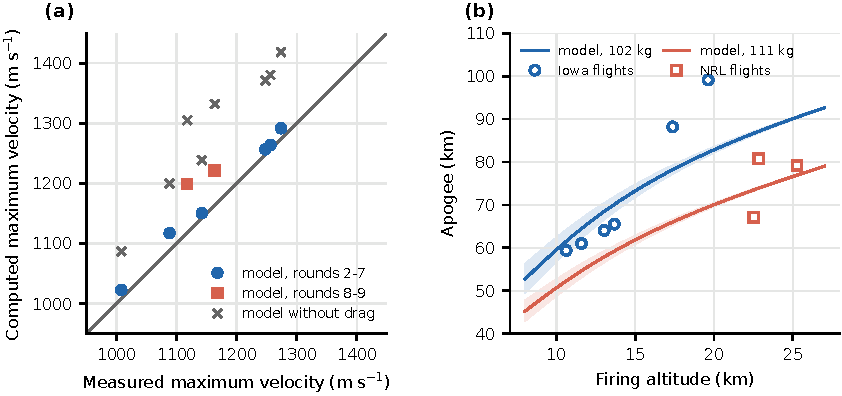
\includegraphics[width=\textwidth]{../paper/figures/fig_validation.pdf}
\caption{Validation. (a) Computed against measured maximum velocity for the eight Deacon ground rounds of Ref.~\cite{watson1949}; crosses show the model with drag switched off. (b) Deacon rockoon flights of 1952--53 \cite{smith1954}: zenith against firing altitude (symbols) and the model with one fitted gross mass per group (lines; bands for drag scale factors of 0.8--1.2).}
\label{fig:validation}
\end{figure}

\begin{table}[!htb]
\centering
\caption{Deacon rockoon firings \cite{smith1954}: firing altitude and zenith from the data sheets, and the apogee computed with one fitted gross mass per group (\R{rkSuiMass}\,kg for the Iowa flights, \R{rkNrlMass}\,kg for the NRL flights).}
\label{tab:rockoons}
\small
\begin{tabular}{lcccc}
\toprule
Flight & Firing altitude (km) & Zenith (km) & Computed (km) & Difference (\%) \\
\midrule
\tabin{../paper/tab_rockoons.tex}
\bottomrule
\end{tabular}
\end{table}

\begin{notes}
\item Baseline: \R{gndAp}\,km and \R{balAp}\,km, ratio \R{gainRatio}. Shares \R{decFDrag}/\R{decFNozzle}/\R{decFHead}\%. Range over switching orders: drag \R{ordDragLo}--\R{ordDragHi}\%, nozzle \R{ordNozzleLo}--\R{ordNozzleHi}\%, head start \R{ordHeadLo}--\R{ordHeadHi}\%.
\end{notes}
\begin{table}[!htb]
\centering
\caption{Baseline vehicle (301.27\,kg gross, 151.27\,kg propellant, diameter 0.40\,m, thrust-to-weight ratio 4, $\eta=0.92$).}
\label{tab:baseline}
\small
\begin{tabular}{lccc}
\toprule
 & Ignition at 30\,km & Ignition at 29\,km & Ground \\
 & from rest & after 1\,km fall & launch \\
\midrule
Nozzle area ratio & \R{balEps} & \R{fallEps} & \R{gndEps} \\
Specific impulse at ignition (s) & \R{balIsp} & \R{fallIsp} & \R{gndIsp} \\
Burn time (s) & \R{balTb} & \R{fallTb} & \R{gndTb} \\
Burnout altitude (km) & \R{balHb} & \R{fallHb} & \R{gndHb} \\
Burnout velocity (m\,s$^{-1}$) & \R{balVb} & \R{fallVb} & \R{gndVb} \\
$\Delta v$ from thrust (m\,s$^{-1}$) & \R{balDv} & \R{fallDv} & \R{gndDv} \\
Gravity loss (m\,s$^{-1}$) & \R{balLg} & \R{fallLg} & \R{gndLg} \\
Drag loss (m\,s$^{-1}$) & \R{balLd} & \R{fallLd} & \R{gndLd} \\
Maximum dynamic pressure (kPa) & \R{balQ} & \R{fallQ} & \R{gndQ} \\
\textbf{Apogee (km)} & \textbf{\R{balAp}} & \textbf{\R{fallAp}} & \textbf{\R{gndAp}} \\
\bottomrule
\end{tabular}
\end{table}

\begin{figure}[!htb]
\centering
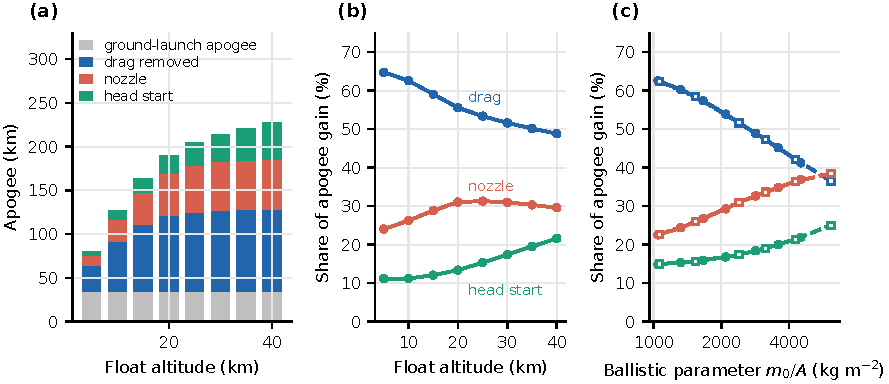
\includegraphics[width=\textwidth]{../paper/figures/fig_decomposition.pdf}
\caption{Decomposition of the apogee gain. (a) Baseline vehicle against float altitude: ground-launch apogee and the three contributions. (b) The same as shares of the gain. (c) Shares at a float altitude of 30\,km against the ballistic parameter. Colours as in (b). Filled symbols: gross mass varied from 25 to 2000\,kg at constant proportions. Open symbols: diameter of the 301\,kg vehicle varied from 0.25 to 0.60\,m.}
\label{fig:decomp}
\end{figure}

\begin{notes}
\item H1: $\Pi_D$ alone gives $R^2$ \R{fitLdOne} for the ground drag loss and \R{fitSdOne} for the drag share; six groups give \R{fitSdFull}.
\end{notes}
\begin{figure}[!htb]
\centering
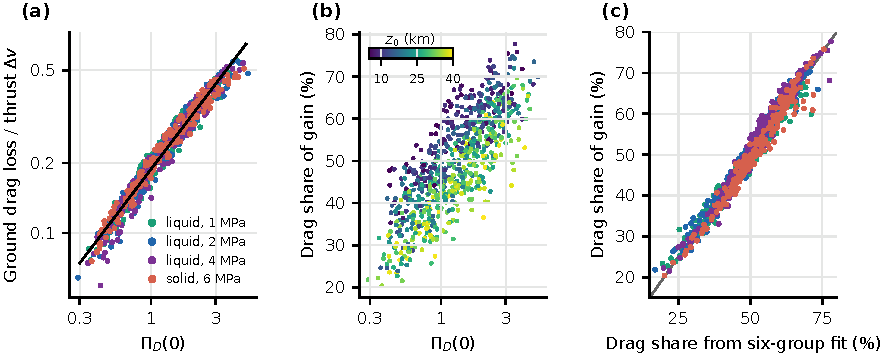
\includegraphics[width=\textwidth]{../paper/figures/fig_collapse.pdf}
\caption{Similarity test over \R{ensN} random vehicles. (a) Drag loss of the ground launch, as a fraction of the thrust $\Delta v$, against $\Pi_D(0)$, coloured by engine; the line is the power-law fit. (b) Drag share of the apogee gain against $\Pi_D(0)$, coloured by float altitude. (c) Drag share against the value given by the six-group fit.}
\label{fig:collapse}
\end{figure}

\begin{table}[!htb]
\centering
\caption{Variance explained ($R^2$) and residual standard deviation of least-squares fits over the ensemble, using $\Pi_D(0)$ alone (quadratic in $\ln\Pi_D$), with $\psi$ and $\xi$ added, and with $p_c/p_0$, $z_0/H$ and $\Pi_c$ added as well. Residuals are in per cent for the logarithmic quantities and in percentage points (pp) for the shares.}
\label{tab:collapse}
\small
\begin{tabular}{lcccccc}
\toprule
 & \multicolumn{2}{c}{$\Pi_D(0)$} & \multicolumn{2}{c}{$+\,\psi,\ \xi$} & \multicolumn{2}{c}{$+\,p_c/p_0,\ z_0/H,\ \Pi_c$} \\
Quantity & $R^2$ & resid. & $R^2$ & resid. & $R^2$ & resid. \\
\midrule
\tabin{../paper/tab_collapse.tex}
\bottomrule
\end{tabular}
\end{table}

\begin{notes}
\item H2: optimum at \R{zsLo}--\R{zsHi}\,km; saving \R{zsSaveLo}--\R{zsSaveHi}\% of launched mass. The predicted dependence on $\ln\Pi_D$ had the wrong sign.
\end{notes}
\begin{figure}[!htb]
\centering
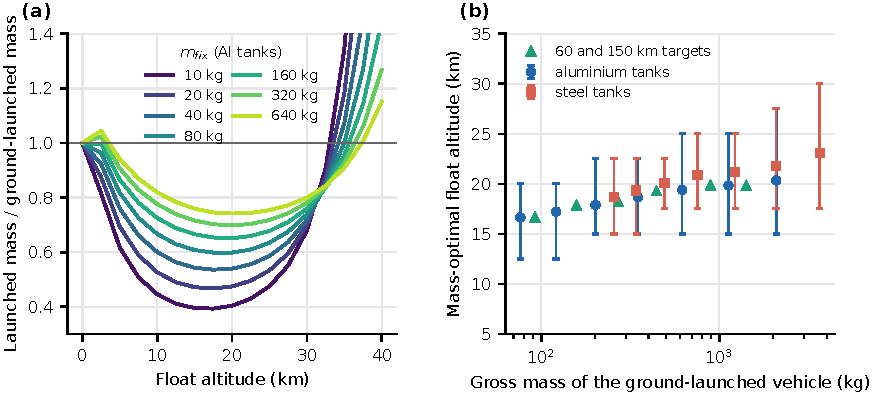
\includegraphics[width=\textwidth]{../paper/figures/fig_optimum.pdf}
\caption{(a) Total launched mass (rocket, gondola, envelope and hydrogen) for a 100\,km apogee, divided by the mass of the ground-launched rocket, against float altitude, for aluminium tanks. (b) Float altitude of minimum launched mass against the mass of the ground-launched vehicle. Bars show the range within 5\% of the minimum.}
\label{fig:optimum}
\end{figure}

\begin{table}[!htb]
\centering
\caption{Mass-optimal float altitude for a 100\,km apogee: ground-launched gross mass, interpolated optimum altitude $z^{*}$, and the launched mass, rocket mass and balloon volume at the nearest computed altitude $z_g$.}
\label{tab:optimum}
\small
\begin{tabular}{cccccccc}
\toprule
Tanks & $m_{\mathrm{fix}}$ & Ground-launched & $z^{*}$ & $z_g$ & Launched mass & Rocket & Balloon \\
 & (kg) & mass (kg) & (km) & (km) & (kg) & (kg) & (m$^3$) \\
\midrule
\tabin{../paper/tab_optimum.tex}
\bottomrule
\end{tabular}
\end{table}

\begin{notes}
\item H3: total-effect index of the drag scale factor \R{sobCdZero} at the ground, \R{sobCdTen} at 10\,km, zero above 15\,km. Monte Carlo: balloon \R{mcBalMed}\,km, ground \R{mcGndMed}\,km (medians).
\item Robustness: fair comparator \R{optRatio}; best over-expanded ground nozzle \R{sepRatio}; build-up drag \R{buRatio}.
\end{notes}
\begin{figure}[!htb]
\centering
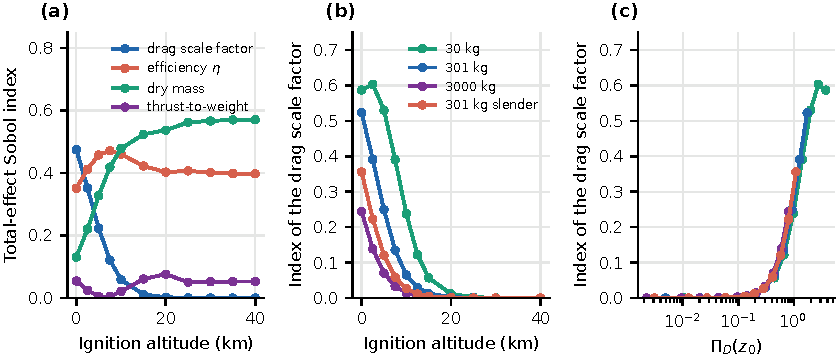
\includegraphics[width=\textwidth]{../paper/figures/fig_sobol.pdf}
\caption{Total-effect Sobol indices of the apogee of the baseline vehicle. (a) Against ignition altitude. (b) Index of the drag scale factor against $\Pi_D(z_0)$.}
\label{fig:sobol}
\end{figure}

\begin{table}[!htb]
\centering
\caption{Sensitivity of the main findings to the assumptions varied in this paper.}
\label{tab:robust}
\footnotesize
\begin{tabular}{@{}>{\raggedright\arraybackslash}p{5.2cm}>{\raggedright\arraybackslash}p{5.6cm}>{\raggedright\arraybackslash}p{3.4cm}@{}}
\toprule
Finding & Varied & Outcome \\
\midrule
Balloon-launched apogee is insensitive to drag & Drag scale 0.5--2; computed build-up curve; Super Loki drag table; Sobol analysis & Robust (changes below 1\%) \\
Ground drag loss scales with $\Pi_D(0)$ & 800 vehicles, four engines; cross-validation & Robust ($R^2=\R{cvLd}$ out of sample) \\
Drag is the largest share of the gain & Float altitude, size, chamber pressure, body shape, drag table, Monte Carlo & Holds in every single-vehicle case except the slimmest body (0.25\,m), where the nozzle share is one point larger; \R{ensDragLargest}\% of the ensemble \\
Mass-optimal float altitude near 20\,km & 14 families, three target apogees, envelope density, gondola fraction & Robust (\R{zsVarLo}--\R{zsHi}\,km) \\
Drag-coefficient uncertainty vanishes above 15\,km & Sobol indices with bootstrap intervals & Robust \\
Apogee ratio of 6.2 for the baseline & Fair comparator (\R{optRatio}); best over-expanded ground nozzle (\R{sepRatio}); build-up drag (\R{buRatio}); Super Loki drag table (\R{acRatio}); tilt & Depends on the set-up \\
Exact shares 52/31/17\% & Chamber pressure, nozzle rule, body shape, drag table & Vary by about ten points \\
Absolute apogees & Efficiency, dry mass, tilt, validation offset of about 6\% & Model outputs only \\
\bottomrule
\end{tabular}
\end{table}

\section*{Discussion}
\begin{notes}
\item Target length: about 900 words. NHSJS parts in order: restatement of key findings; implications and significance; connection to objectives; recommendations; limitations; closing thought. No new information here.
\item Connection to objectives: H1 holds for the drag loss and fails for the shares; H2 holds for existence and fails for the predicted trend; H3 holds.
\item Limitations to state: first-order model; liquid engine not flight-validated; one fitted mass per rockoon group; the two drag checks disagree (ground firings fit \R{deaCdFit}, rockoon flights prefer about 2); nozzle mass not counted; no wind, pointing or cost.
\item Recommendations: a measured or computed drag curve for a defined vehicle; flight data for a liquid rockoon; a six-degree-of-freedom launch model.
\end{notes}

\section*{Acknowledgments}
\begin{notes}
\item Leave empty in the review copy. Add names only in the final version.
\end{notes}

\section*{AI use statement}
\begin{notes}
\item NHSJS wants this after the Acknowledgments and before the References. Name each tool and what it was used for. It must be true of the version you submit.
\end{notes}

\ifonline\else
\begin{thebibliography}{99}
\input{bib_order.tex}
\end{thebibliography}
\fi
\end{document}
